\section{Functions}
Functions are simply pre-written code frgaments that perform a certain task.\footnote{In older procedure languages functions and subroutines are similar, but a function returns a value whereas a subroutine operates on data.  The difference is subtle but important.   More recent thinking has functions being able to operate on data (they always could) and the value returned may be simply an exit code.} 
An analogy are the functions in MS Excel. To add numbers, we can use the \texttt{sum(\textsl{range})} function and type \texttt{=sum(A1:A5)} instead of typing \texttt{=A1+A2+A3+A4+A5}

We call a function simply by typing the name of the function or by using the dot notation.\footnote{Whether we can use the dot notation or not depends on how the function is written, whether it is part of a class, and how it is imported into a program.} 
Some functions require us to pass data in for them to perform their tasks. 
These data are known as arguments\footnote{or argument list} and we pass them to the function by enclosing their values in parenthesis ( ) separated by commas. � 
For instance,  the \texttt{print()} function for displaying text on the screen is ``called''  by typing \texttt{print(``Hello World'')} where \texttt{print} is the name of the function and \texttt{``Hello World''} is the argument.

\subsection{User defined functions}
We can define our own functions in \textbf{Python} and reuse them throughout the program. 

The syntax for defining a function is: � 
\begin{verbatim}
def functionName( argument ): 
      code detailing what the function should do
      return [expression] � 
\end{verbatim}

The keyword~\texttt{def} tells the program that the indented code from the next line onwards is part of the function. 
The keyword~\texttt{return} tells the program to return an answer from the function. 
There can be multiple return statements in a function. Once the function executes a return statement, the program exits the function and continues with its next executable statement. 
If the function does not need to return any value, you can omit the return statement.\footnote{I would consider this bad programming practice because the code would become hard to maintain,  alternatively, you can write \texttt{return} or \texttt{return None}, which would be a better programming style.}

Functions can be pretty elaborate -- they can search for things in a list, determine variable types, open and close files, read and write to files.   To get started we will build a few really simple mathematical functions --- we will need this skill in the future anyway, especially in scientific programming contexts.

For our first function we will code $f(x) = x \sqrt{1+x}$ into a function named \texttt{dusty}
\begin{verbatim}
def dusty(x) :
     temp = x * ((1.0+x)**(0.5)) # should use the math package 
     return temp
# the function should make the evaluation
# store in the local variable temp
# return contents of temp
\end{verbatim}

Figure \ref{fig:MyFirstFunction} is a screen capture of the code (without the comments) and a couple of runs of the module.  Notice we included error trapping (because its easy using cut and paste from code in earlier chapters).

\begin{figure}[htbp] %  figure placement: here, top, bottom, or page
   \centering
   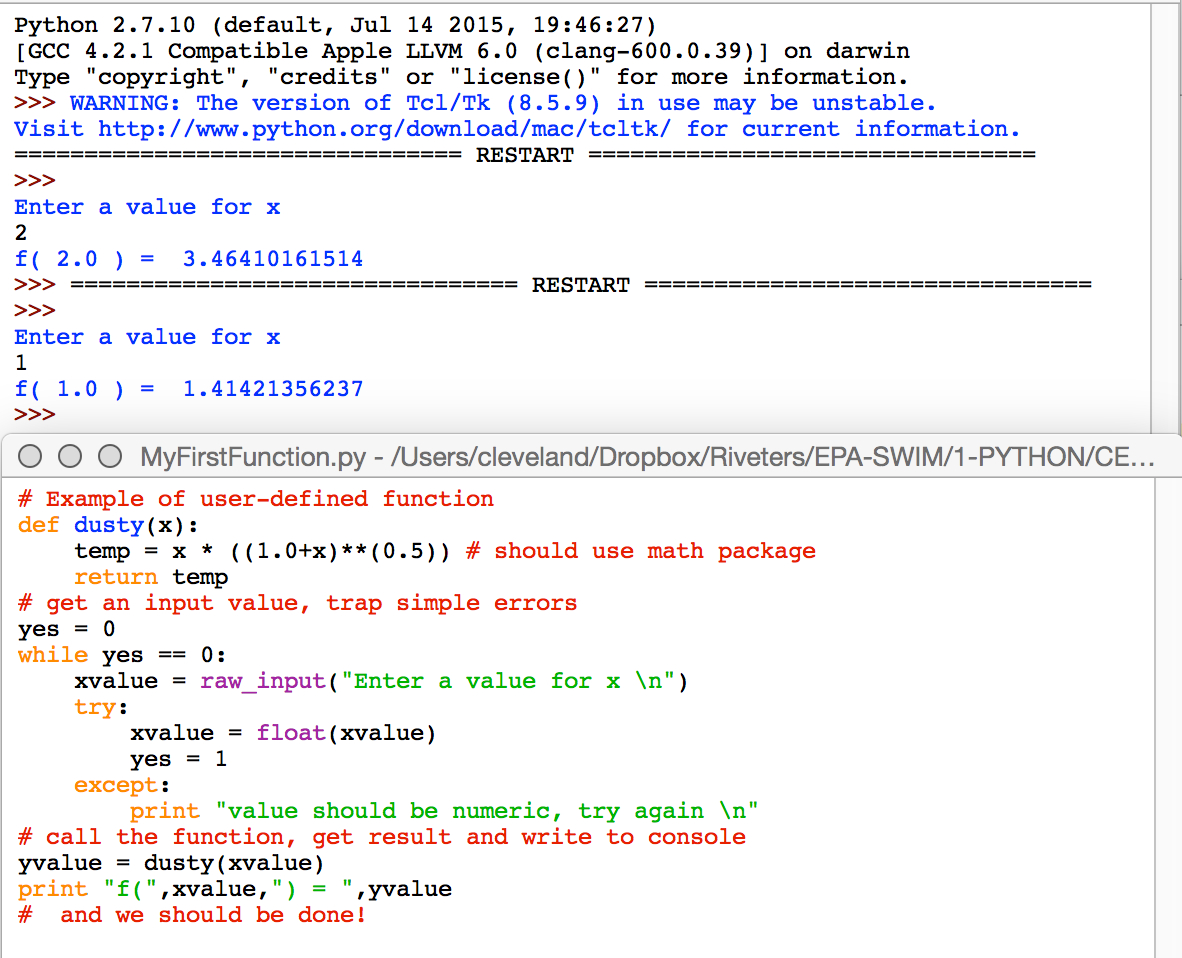
\includegraphics[width=5in]{./10-Functions/MyFirstFunction.jpg} 
   \caption{The function \texttt{dusty()} coded and run in \textbf{Python}.}
   \label{fig:MyFirstFunction}
\end{figure}

\subsubsection{Variable Scope} � 
An important concept when defining a function is the concept of variable scope. 
Variables defined inside a function are treated differently from variables defined outside. 
Firstly, any variable declared within a function is only accessible within the function. These are known as local variables. 
In the \texttt{dusty()} function, the variables \texttt{x} and \texttt{temp} are local to the function.  Any variable declared outside a function in a main program is known as a global variable and is accessible anywhere in the program.  In the example, the variables \texttt{xvalue} and \texttt{yvalue} are global (to the program -- if they are addressed within a function, they could be operated on.  Generally we want to protect the global variables from the function unless the intent is to change their values.   The way the function is written in the example, it [the function] cannot damage \texttt{xvalue} or \texttt{yvalue}.

If a local variable shares the same name as a global variable, any code inside the function is accessing the local variable. 
Any code outside is accessing the global variable.\footnote{A good style is to keep names different --- sometimes its hard to do when multiple programmers are working on the same code modules.   Usually a coding project agrees ahead of time on some naming convention so multiple programmers can work on different parts of the program without damaging the overall program.   This convention is especially important when refactoring (rewriting) legacy programs.}

\subsection{Importing Modules}
\textbf{Python} is distributed with a large number of built-in functions. 
These functions are saved in files known as modules. 
To use the built-in codes in Python modules, we have to import them into our programs first. 
We do that by using the \texttt{import} keyword. 
There are three ways to import:� 
\begin{enumerate}
\item Import the entire module by writing \texttt{import moduleName}; For instance, to import the random module, we write \texttt{import random}.
To use the \texttt{randrange()} function in the random module, we write \texttt{random.randrange( 1, 10)};\footnote{The syntax is \texttt{moduleName.functionName(argument\_list)}.}

\item Import and rename the module by writing \texttt{import random as r} (where r is any name of your choice). Now to use the \texttt{randrange()} function, you simply write \texttt{r.randrange( 1, 10)}; and

\item Import specific functions from the module by writing \texttt{from moduleName import name1[, name2[, ... nameN]]}. � 
For instance, to import the \texttt{randrange()} function from the random module, we write \texttt{from random import randrange}. 
To import multiple functions, we separate them with a comma. 
To import the \texttt{randrange()} and \texttt{randint()} functions, we write \texttt{from random import randrange, randint}. To use the function now, we do not have to use the dot notation anymore. Just write \texttt{randrange( 1, 10)}.

\end{enumerate}

\subsubsection{User built modules}
Besides importing built-in modules, we can also create our own modules. 
We will find this concept useful (if not vital) when we have functions that we want to reuse in other programming projects in future. � 
Creating a module is simply accomplished by saving the file with a .py extension and put it in the same folder as the Python file that you are going to import it from.\footnote{Alternatively put it in a static location and when you import provide the entire absolute path name to the file.  In practice I imagine one would adopt both models for distributing programs.  Keep really solid code in an absolute location, but distribute copies with localized modules so the end user does not need to mess with paths.}

As an example, we will modify the code to have a main program and a module called \texttt{MyFunctionsModule}.

\begin{figure}[h!] %  figure placement: here, top, bottom, or page
   \centering
   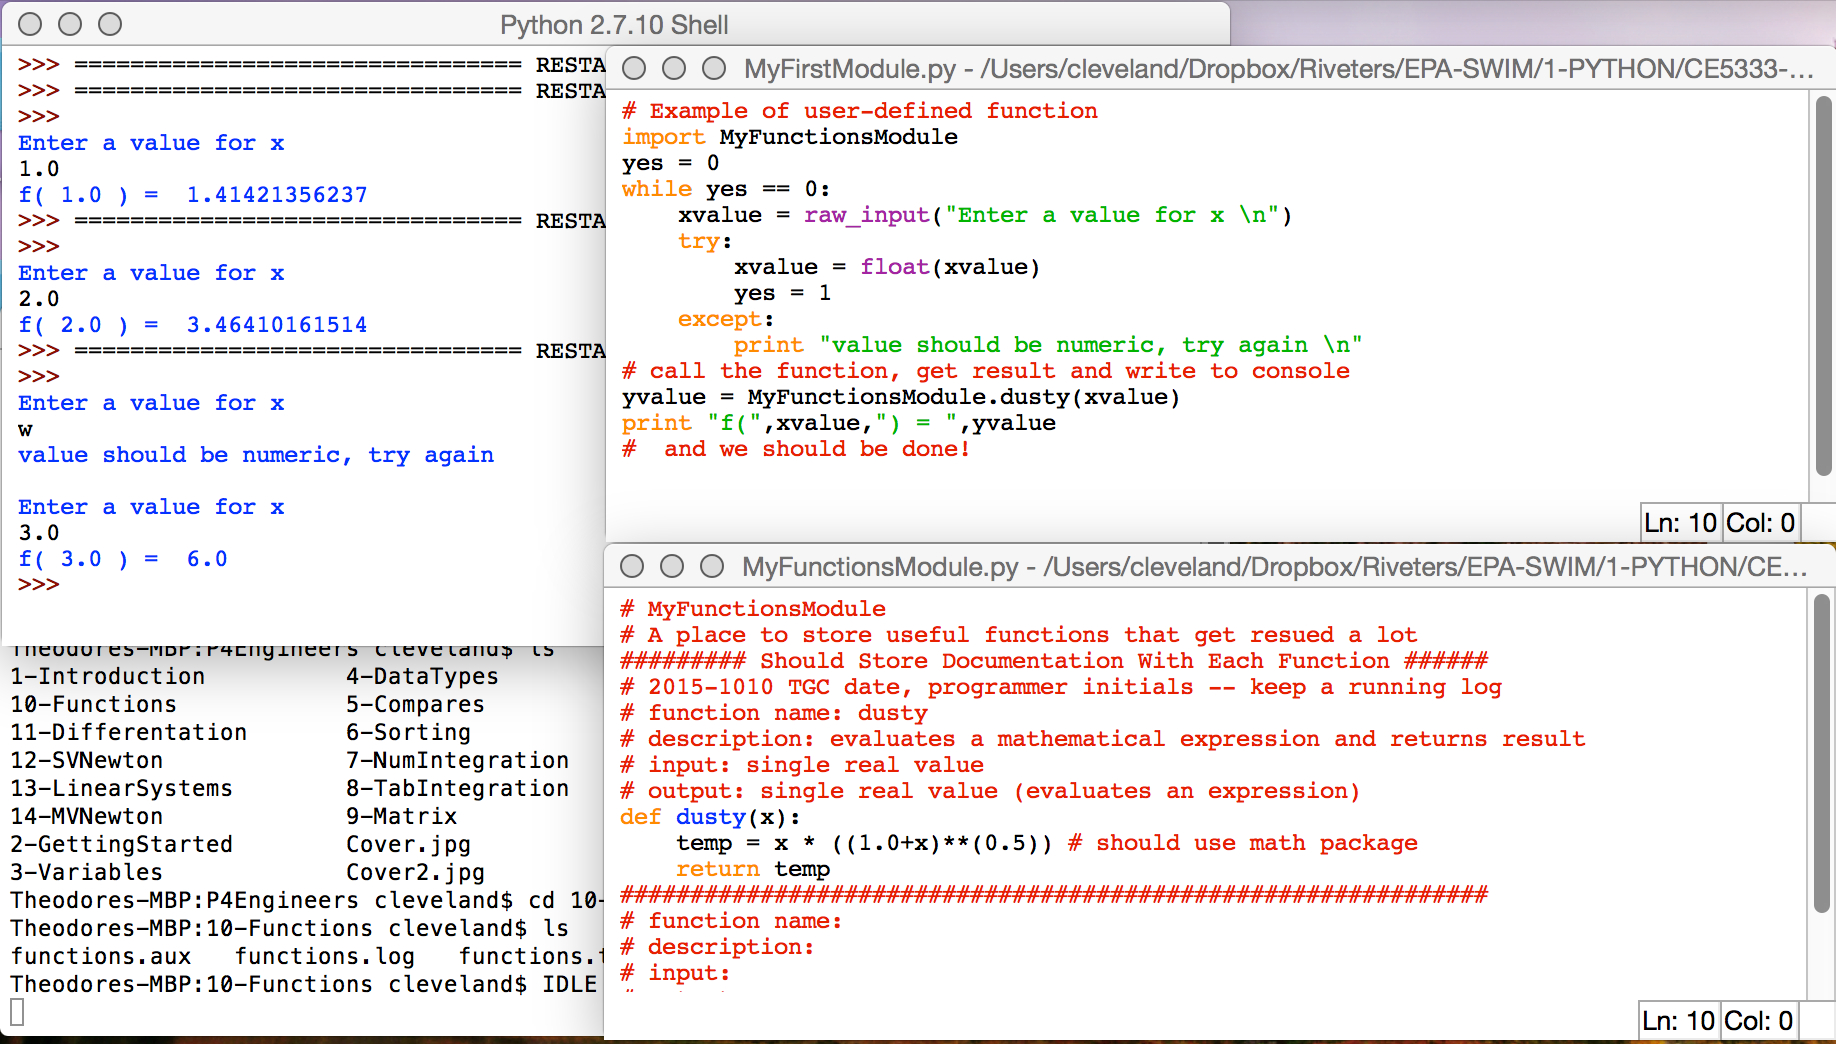
\includegraphics[width=6in]{./10-Functions/MyFunctionModule.jpg} 
   \caption{The \texttt{dusty()} function stored in a module and called from a program by importing the module.  Notice the need for the module name and the function name using the dot syntax.}
   \label{fig:MyFunctionModule}
\end{figure}

\subsection{Built-In Modules and Packages}
The modules that come with \textbf{Python} are extensive and listed at \url{https://docs.python.org/2/py-modindex.html}.  
There are also other modules that can be downloaded and used (just like user defined modules).  
Probably one that will be useful after we are done with primitive programming is  the \texttt{NumPy} package \url{http://www.numpy.org}.

In this document we are building primitive codes to learn how to code and how to create algorithms.   For many practical cases you will want to load a well-tested package to accomplish the tasks.  That exercise is saved for the end of the document.

\subsection{}






